
\documentclass[12pt,a4paper]{article}
\usepackage[a4paper, total={6.7in,8.1in}]{geometry}
\usepackage{color}
\usepackage{graphicx}

%\usepackage{geometry}
%\geometry{legalpaper, landscape, margin=2in}
\usepackage[utf8]{inputenc}
\usepackage{multicol}
%\graphicspath{ {home/yoshimar/Escritorio/} }
\setlength{\columnsep}{1cm}
\title{Aproximaciones Gausssianas:\\Normal, Binomial y Poisson}
\author{Condori Muñoz Rommel Yoshimar}


\date{Diciembre 2018}

\begin{document}

\maketitle
\begin{multicols}{2}
\section{Resumen}
    En el presente proyecto se verá el comportamiento de las distribuciones Normal,Binomial y Poisson, y su relación entre éstas por medio de aproximaciones en una simulación  que se ha de dar por medio de Python.
\section{Introducción}
    Las variables aleatorias han llegado a desempeñar un papel importante en casi todos los campos de estudio: en la Física, la Química y la Ingeniería; y especialmente en las ciencias biológicas y sociales. Estas variables aleatorias son medidas y analizadas en términos de sus propiedades estadísticas y probabilísticas, de las cuales una característica subyacente es su función de distribución. A pesar de que el número potencial de distribuciones puede ser muy grande, en la práctica, un número relativamente pequeño se utilizan; ya sea porque tienen características matemáticas que las hace fáciles de usar o porque se asemejan bastante bien a una porción de la realidad, o por ambas razones combinadas.
    
    En ocasiones, algunas variables aleatorias siguen distribuciones de probabilidad muy concretas, como por ejemplo el estudio a un colectivo numeroso de individuos que se modelizan por la distribución “Normal”. Veremos sólo algunas de las distribuciones o modelos de probabilidad más importantes como son las aproximaciones Gaussianas que se dan para las distribuciones Poisson,Binomial(discretas) y Normal(continua)   y que después nos resultarán muy útiles como por ejemplo para el tema de la Estimación.
    Como hemos visto, las variables pueden ser discretas o continuas; por ello, también las distribuciones a tratar podrán ir asociadas a variables aleatorias discretas o continuas.\\
    \\ \textbf{Distribución Poisson.} La Distribución Poisson esta dada por la fórmula:
    $$\rho(r;\mu)=\frac{\mu^re^{-\mu}}{r!}$$
    
    En dónde $r$ es un entero $r\geq0$ y $\mu$ es un número real positivo. La Distribución Poisson describe la probabilidad de encontrar exactamente r eventos en un lapso de tiempo si los acontecimientos se producen de forma independiente a una velocidad constante μ. Es una de las distribuciones más utilizadas en estadística con varias aplicaciones; como por ejemplo describir el número de fallos en un lote de materiales o la cantidad de llegadas por hora a un centro de servicios.\\\\
    \textbf{Distribución Binomial.} La Distribución Binomial esta dada por la fórmula: 
    $$\rho(r;N,p)={N \choose r}p^r(1-p)^{N-r}$$
    
    En dónde $r$ con la condición $0\leq r\leq N$ y el parámetro $N$ ($N>0$) son enteros; y el parámetro $p$ ($0\leq p\leq1$) es un número real. La Distribución Binomial describe la probabilidad de exactamente $r$ éxitos en $N$ pruebas si la probabilidad de éxito en una sola prueba es $p$. 
    \\ \textbf{Distribución Normal.} La Distribución Normal, o también llamada Distribución de Gauss, se caracteriza porque los valores  se distribuyen  formando una campana de Gauss, en torno  a un valor central que coincide con el valor  medio de la distribución, es aplicable a un amplio rango de problemas, lo que la convierte en la distribución más utilizada en estadística; esta dada por la formula:
    $$\rho(x;\mu,\sigma^2)=\frac{1}{\sigma\sqrt{2\pi}}\epsilon^{-\frac{1}{2}(\frac{x-\mu}{\sigma})^2}$$
    
    En dónde $\mu$ es el parámetro de ubicación, y va a ser igual a la media aritmética y $\sigma^2$ es el desvío estándar. Algunos ejemplos de variables asociadas a fenómenos naturales que siguen el modelo de la Distribución Normal son:
    \begin{itemize}
        \item Características morfológicas de individuos, como la estatura;
        \item Características sociológicas, como el consumo de cierto producto por un mismo grupo de individuos;
        \item Características psicológicas, como el cociente intelectual;
        \item Nivel de ruido en telecomunicaciones;
        \item Errores cometidos al medir ciertas magnitudes;
        \item etc.
    \end{itemize}
    
    
    [1] [2]
    
    
    
    
\section{Estado del arte}
    Algunos artículos relacionados al tema:
    \begin{itemize}
        \item \textbf{Clasificación de eventos sísmicos empleados  procesos gaussianos}: La clasificación de señales es de crucial  importancia para el descubrimiento de posibles interacciones entre movimientos telúricos volcánicos per se. En este artículo  se presenta la aplicación de procesos gaussianos para la clasificación de eventos sísmicos registrados en un nevado en partilar.Las señales se caracterizan usando los coeficientes  de un modelo autoregresivo, empleado para estimar la densidad espectral de potencia. La función de distribución predictiva para la clasificación se aproxima mediante el método de Laplace.El desempeño obtenido es mayor que el de una red neuronal artificial, clasificador  utilizado tradicionalmente para resolver una tarea.[3]\\
        \item \textbf{Discontinuidad en la BMV: Aplicando Procesos Poisson-Gaussianos a los Activos Nacionales. Desechando la Distribución Normal}:La administración de riesgos actual se divide en tres grandes temas: el cálculo de productos derivados, la modelación de las tasas de interés y el área de riesgos financieros y económicos.Específicamente, desde los trabajos realizados por Bachelier(1900), la modelación financiera ha involucrado la presencia del movimiento Browniano. Lo anterior nos conduce a mantener supuestos que incluyen desde comportamientos log normales por parte de los rendimientos de los activos hasta varianzas que no son proporcionales al tiempo. Este trabajo propone el uso de una distribución diferente a la distribución normal para la teoría financiera utilizando los rendimientos de un grupo de activos nacionales. Se trata del uso del modelo Poisson-Gaussiano. Se aplica una aproximación propuesta por Sanjiv Das (1998) en la obtención de la función de verosimilitud para el caso de once activos pertenecientes a la BMV y sus series correspondientes del10 de enero del 1994 al 31 de diciembre del 2004.[4]\\
        \item \textbf{Aproximación mediante Gaussianas  de datos electroforéticos}: La electroforesis capilar (EC) es una técnica de separación y análisis de sustancias químicas ampliamente utilizada en la industria biotecnológica y bioquímica. El resultado del análisis de una muestra química con EC es una señal llamada electroferograma donde varios picos  representan los distintos subcomponentes de la muestra. La forma de cada pico, bajo condiciones determinadas, puede modelarse con una función gaussiana, aunque  frecuentemente los picos  pueden presentar importantes deformaciones en su forma ideal debido a procesos físico-químicos que ocurren  dentro del capilar. Estas formas  no son exactamente  gaussianas pueden ser modeladas con otras funciones que llamamos gaussianas modificadas. El objetivo del trabajo  fue la obtención  de los parámetros que definen a cada gaussiana, modelando a su vez  las prolongaciones de los picos ("tailing") mediante gaussianas modificadas. Se realiza un proceso de análisis  previo mediante transformada waveleis discreta para las disminución de ruido y la reducción de la dimensión de los datos, y adicionalmente se aplica un algoritmo de corrección de línea base. Se calculan los parámetros iniciales de las gaussianas (ubicación, amplitud, ancho) y finalmente se realiza la aproximación  definitiva de la  curva compuesta  por sumas gaussianas  a la señal original  mediante un proceso  de optimización no lineal (región de confianza). El beneficio  práctico  de la descomposición en suma de gaussianas  de la señal electroforética se aprecia de manera relevante en cuanto a la  significativa reducción en la cantidad de datos  al 0.47\%, ideal para manejar los sistemas emergentes de recolección  de muestras químicas de alta resolución en tiempo y de electroforesis multicapilar, los cuales generan grandes cantidades de  datos en muy poco tiempo.[5]
    \end{itemize}
\section{Diseño del experimento}
    
    En Python se pudo generar fácilmente con la ayuda de \textbf{scipy.stats}, paquete que utilizamos para representar a todas las  distribuciones  en cuestión a lo largo del artículo, de este paquete en específico las siguientes funciones:
    \begin{itemize}
        \item scipy.stats.\textbf{poisson}, La función de masa de probabilidad lo define en la forma "estandarizada". Para cambiar la distribución se usa el parámetro loc. Específicamente, poisson.pmf (k, mu, loc) es idénticamente equivalente a poisson.pmf (k - loc, mu).
        \item scipy.stats.\textbf{binomial}, La función de masa de probabilidad se define en la forma "estandarizada". Para cambiar la distribución se usa el parámetro loc. Específicamente, binom.pmf (k, n, p, loc) es idénticamente equivalente a binom.pmf (k - loc, n, p).
        \item scipy.stats.\textbf{normal}, La densidad de probabilidad se define en la forma "estandarizada". Para cambiar y/o escalar la distribución, use los parámetros loc y scale. Específicamente, norm.pdf (x, loc, scale) es idénticamente equivalente a norm.pdf (y) / scale con y = (x - loc) / scale.
    \end{itemize} 
    Adicionalmente hacemos uso del paquete \textbf{matplolib} para generarnos los gráficos.
    
\section{Experimentos y resultados}
    A continuación se muestra las gráficas de las distribuciones:\\
    (https://github.com/ycmunoz/proyecto-estadistica/blob/master/gauss.ipynb)
    \begin{itemize}
        \item \textbf{Distribución Poisson}\\
        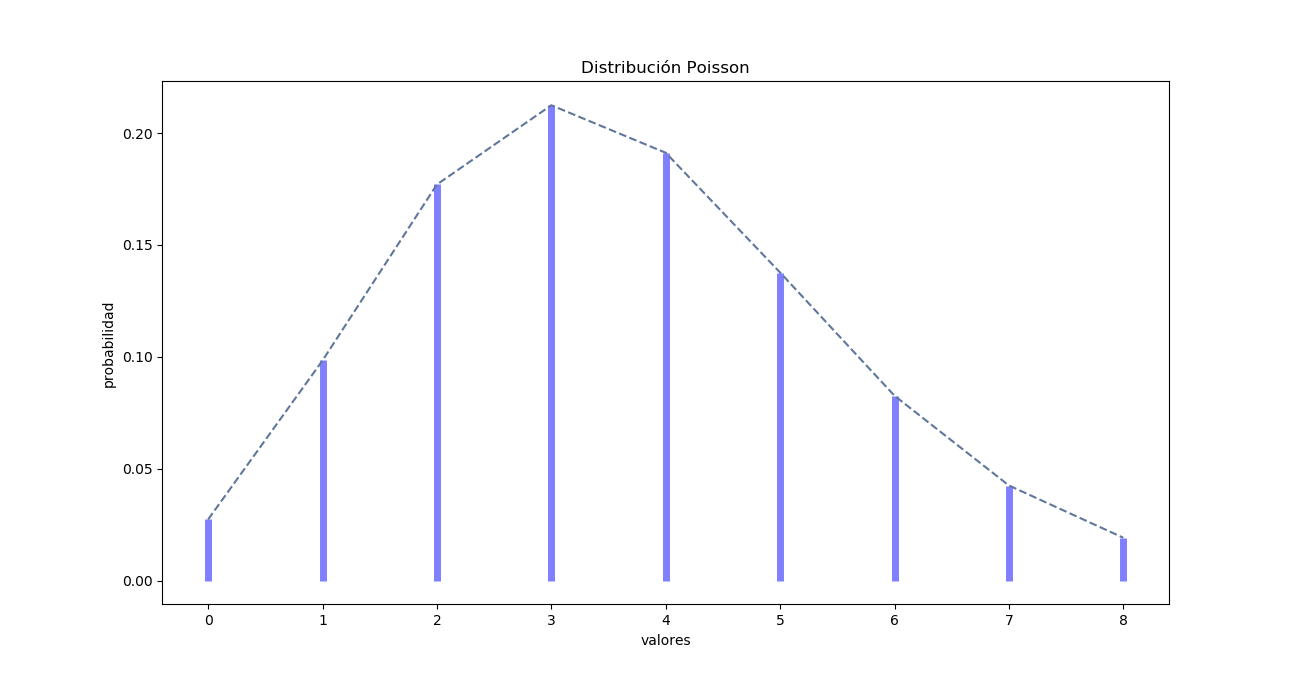
\includegraphics[scale=0.26]{poisson.png}
        \item \textbf{Distribución Binomial}\\
        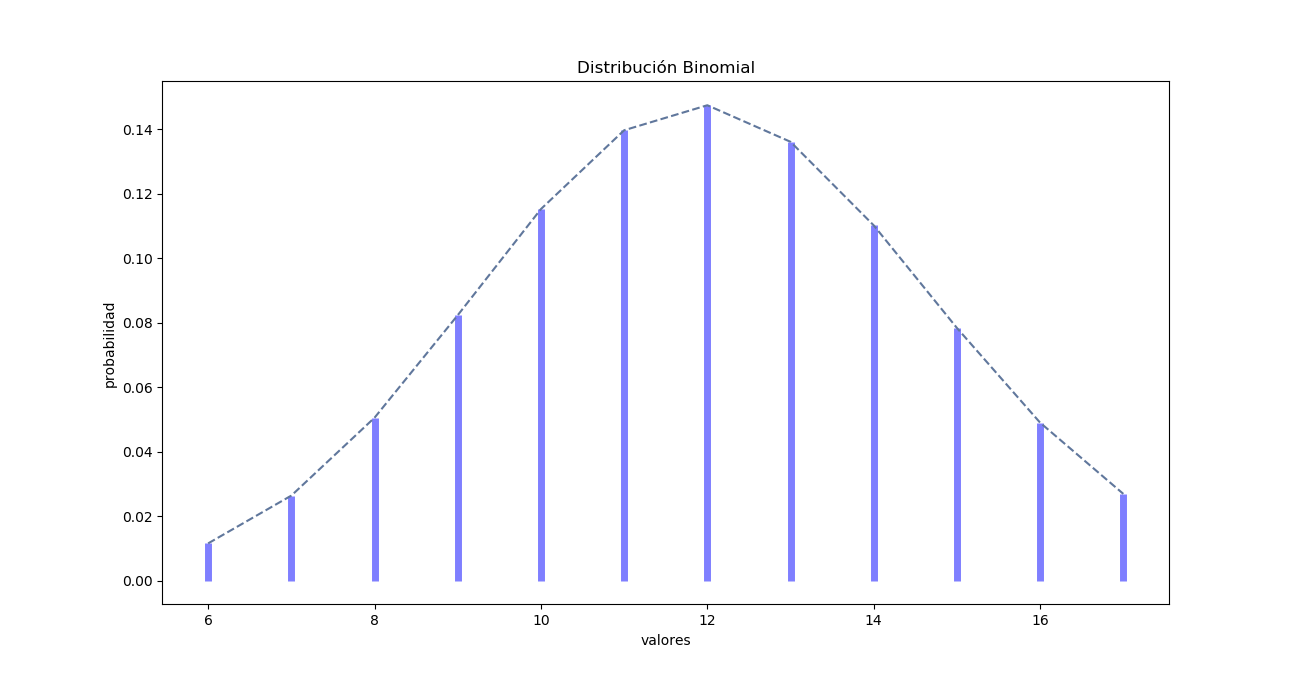
\includegraphics[scale=0.26]{binomial.png}
        \item \textbf{Distribución Normal}\\
        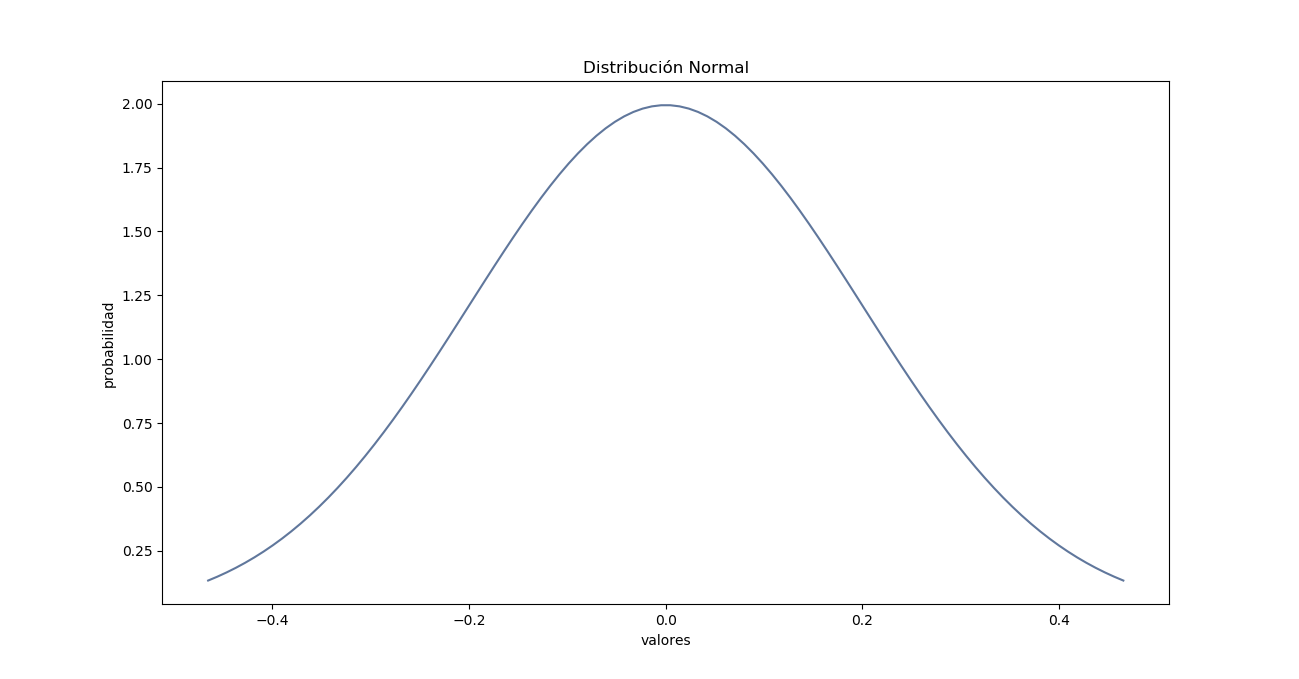
\includegraphics[scale=0.26]{normal.png}
    \end{itemize}
    \\\\Ahora,las \textbf{aproximaciones Gaussianas:}
    \begin{itemize}
        \item \textbf{Poisson-Normal:}\\
        En el programa aumento el parámetro mu.\\
        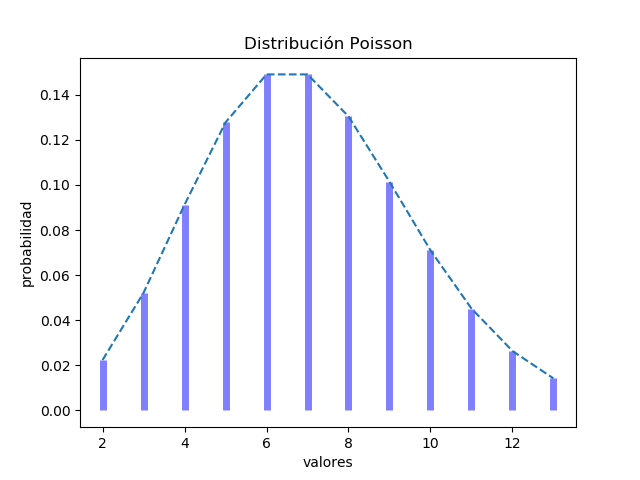
\includegraphics[scale=0.50]{poisson_normal_1.png}
        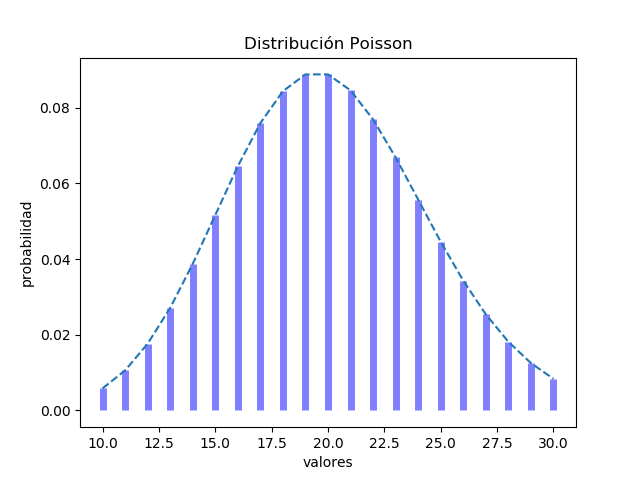
\includegraphics[scale=0.5]{poisson_normal_2.png}
        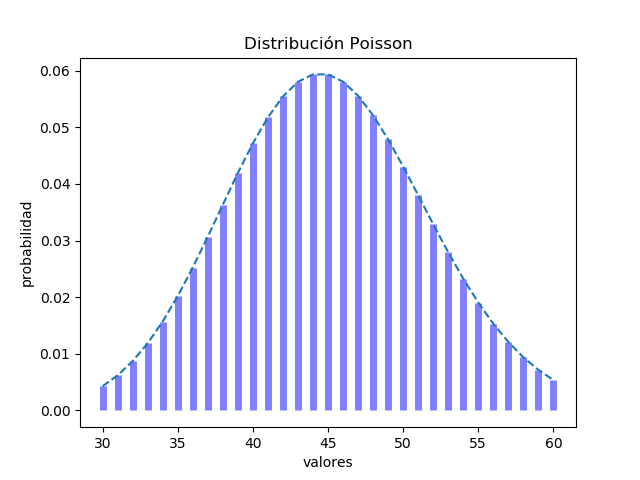
\includegraphics[scale=0.5]{poisson_normal_3.png}
        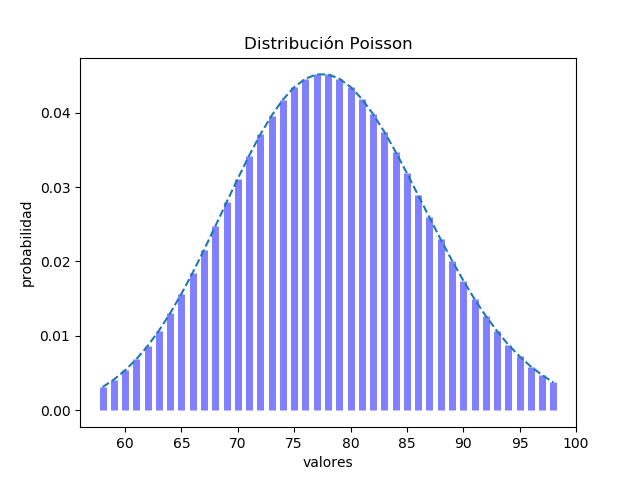
\includegraphics[scale=0.5]{poisson_normal_4.png}
        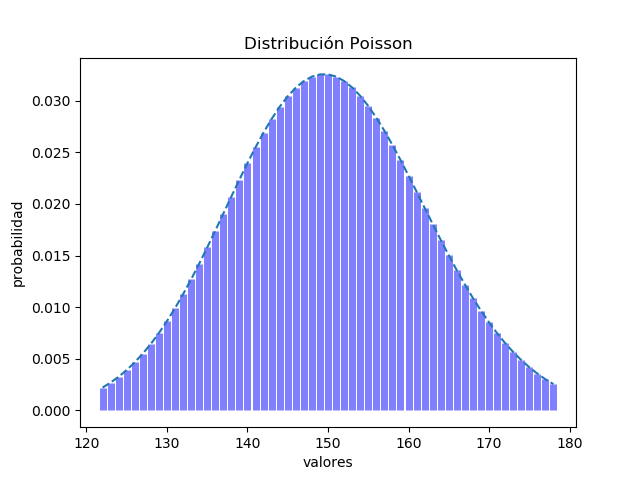
\includegraphics[scale=0.5]{poisson_normal_5.png}
    \end{itemize}
    \begin{itemize}
        \item \textbf{Binomial-Normal:}\\
        En el programa aumento el valor N y dejo constante el valor p=0.5\\
        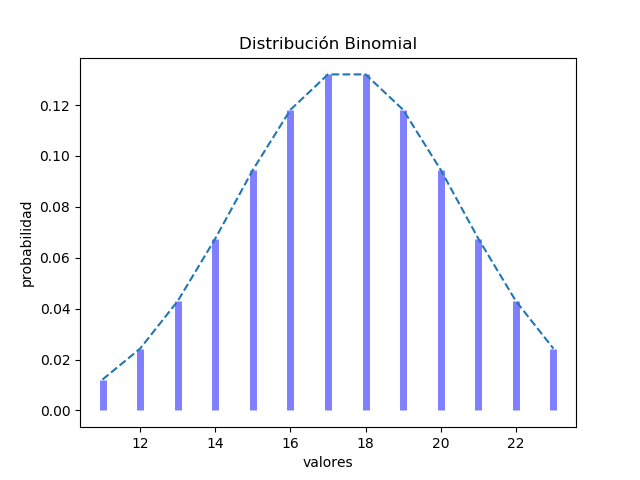
\includegraphics[scale=0.5]{binomial_normal_1.png}
        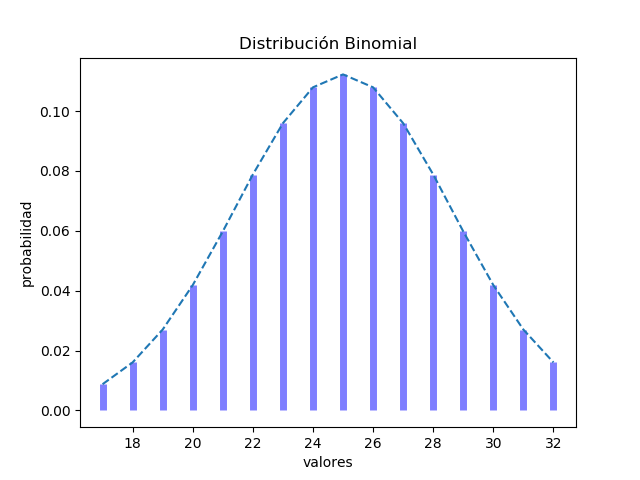
\includegraphics[scale=0.5]{binomial_normal_2.png}
        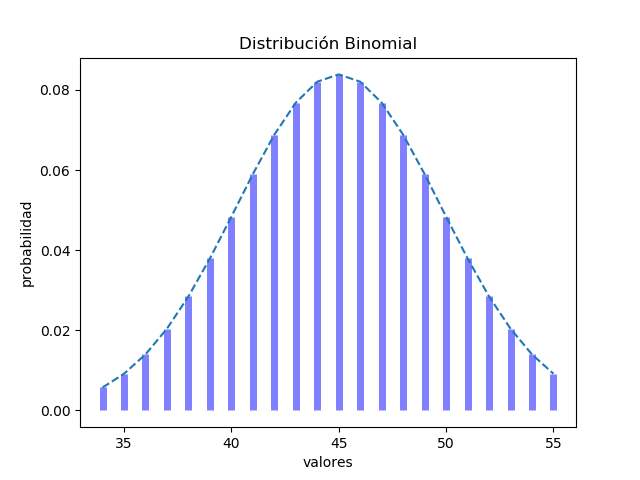
\includegraphics[scale=0.5]{binomial_normal_3.png}
        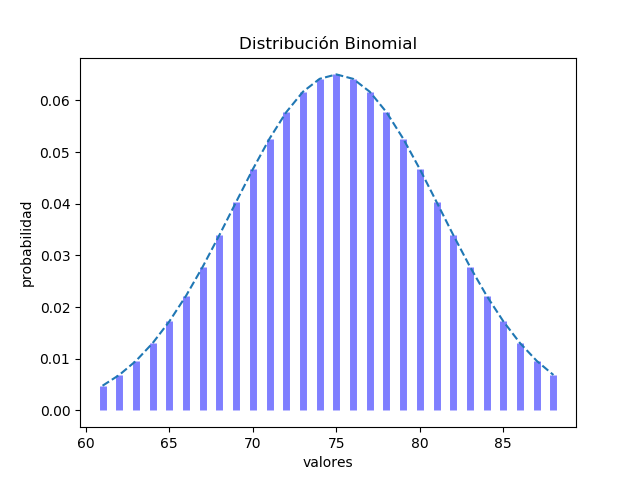
\includegraphics[scale=0.5]{binomial_normal_4.png}
    \end{itemize}
\section{Conclusiones}
    Se observa de las gráficas el comportamiento bajo las condiciones dadas:\\
    La \textbf{aproximación Poisson-Normal} se da como consecuencia del \textit{Teorema Central del Límite}, para valores grandes de $\mu$, una variable aleatoria de Poisson $X$ puede aproximarse por otra Normal dado que el cociente:
    $$Y=\frac{X-\mu}{\sqrt{\mu}}$$
    converge a una districión Normal de media 0 y de varianza 1.\\
    La \textbf{aproximación Binormal-Normal} se cumple cuando $p=0.5$ y $N$ es muy grande(usualmente se exige que $N\geq30$), la distribución Binomial puede aproximarse mediante la distribución Normal.
    
    Las gráficas son similares a las teóricas, lo cual dice que se ha simulado bien el experimento, quizá en el de las distribuciones de Poisson y Binomial faltó extender mas la gráfica en el eje X+ para ver la totalidad de ésta, dejamos al lector notar ésta acotación. 
\section{Bibliografía}
\begin{enumerate}
    \item Montero Alonso, Miguel Ángel, (2007), Apuntes de Estadística II, Granada-España, Editorial Universidad de Granada , pag. 33-44.
    \item Robert V. Hogg, Allen Craig, Joseph W. Mackean,2004 Introductions to Mathematical Stadistics. 6ta Ed., Editorial Pearson, pag 133-160. 
    \item Alvarez,M ,Henao,R ,Duque,E (2007) , Scientia et Technica, No.35, pag. 145-150.
    \item Moreno Quezada, Guillermo E., (02-09-2016), Discontinuidad en la BMV: Aplicando Procesos Poisson-Gaussianos a los Activos Nacionales. Desechando la Distribución Normal., Instituto Tecnológico y de Estudios Superiores de Monterrey, Monterrey- México.
    \item Ceballos,Gerardo A., (2010), Aproximación mediante Gaussianas de datos electroforéticos, Universidad de Los Andes, Mérida-Venezuela.
\end{enumerate}
\end{multicols}
\end{document}
